\documentclass[12pt]{article}

\usepackage{commondoc}
\usepackage{circuitikz}
\usepackage{chngcntr}

% because of polyglot...
\usepackage{luatexja-fontspec}
\setmainjfont{SimHei}


% hmm.
\makeatletter\@removefromreset{section}{part}\makeatother
\counterwithin{figure}{section}
\counterwithin{listing}{section}

\hypersetup{
	pdftitle={[CDDC19]-S4F3 S0L1D5},
	pdfauthor={Team S4F3 S0L1D5},
	colorlinks=true,
	linkcolor=MidnightBlue,
	urlcolor=MidnightBlue,
}

\NewDocumentCommand{\ttt}{m}{\texttt{#1}}
\NewDocumentCommand{\cddcflag}{m}{\textcolor{Maroon}{\ttt{\$CDDC19\$\{#1\}}}}
\NewDocumentEnvironment{multipagecode}{}{\captionsetup{type=listing}}{}

% ok, so this isn't meant for print; we ignore the odd-page rule for parts by just re-defining \ensureoddpage
% to do nothing.
\renewcommand{\ensureoddpage}{}



\title{CDDC 2019 Qualifiers}
\author{Team S4F3 S0L1D5}

\begin{document}
\pagenumbering{gobble}
\hypersetup{pageanchor=false}
\begin{center}

	\vspace*{5mm}

	\begin{flushleft}

	{
		\Roboto\fontsize{36pt}{48pt}\selectfont CDDC 2019 Qualifiers \\
		\Roboto\fontsize{28pt}{40pt}\selectfont Challenge Writeup

		\vfill

		\normalfont\fontsize{20pt}{24pt}\selectfont Team:    \tabto{30mm} \fontsize{24pt}{24pt}\selectfont \texttt{S4F3 S0L1D5} \\
		\normalfont\fontsize{20pt}{24pt}\selectfont Category:\tabto{30mm} Uni/Poly

		\vspace{5mm}
		\normalfont\fontsize{16pt}{20pt}\selectfont June 2019
		\vspace{30mm}
	}

	\end{flushleft}


\end{center}


\pagebreak
\pagenumbering{arabic}
\hypersetup{pageanchor=true}


\pagebreak\part{OSINT\_RED}
% r0, r1, r2, r3-1, r4-1, r4-1-2

\section{[R-0] Everyone <3 Fan Mail}

	This series of challenges were made slightly more tedious than necessary, because unfortunately there was a real company
	called \enquote{LightSpeed} that diluted the search results.

	The main objective of this challenge was to find the email of the site administrator for \url{www.lightspeedcorp.global}, and
	send him an email.

	\subsection{Solution}

		In theory, all we would have needed to do was perform a WHOIS lookup on the domain to find the email address. Simple,
		right?

		Nope.

		Depending on which WHOIS search engine is used, certain bits of information about the registrant can be missing if the
		domain was registered with WHOISGuard, which hides certain identifiable information from WHOIS lookups.

		\begin{figure}[!htbp]\centering
			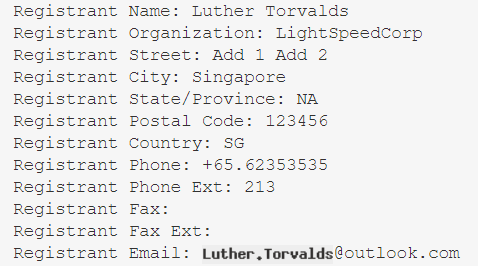
\includegraphics[width=110mm]{figures/osintred/r0.png} \vspace{5mm}
			\caption{All the information is visible if WHOISGuard is ignored}
		\end{figure}

		\pagebreak
		However, it turns out that the guard isn't perfect, and all we had to do was find a WHOIS search engine that ignores the
		guard. After some digging, we found one, exposing all the juicy details of the registrant.

		After getting the email address, we just had to send an email, and we were replied with the flag.

	% end subsection

	\subsection{Flag}
		The flag for this challenge was \cddcflag{IS\_IT\_I\_AM\_FAM0US\_NAO}.
	% end subsection

% end section


\pagebreak
\section{[R-1] Travel to the Past}

	The challenge heavily hinted that we would need a way to look at an older version of the website to find the flag, and that's exactly
	what we did.

	\subsection{Solution}

		There was a single snapshot of the website on the Wayback Machine\footnote{\url{https://archive.org/web/}} on the 20\sps{th} of May,
		and browsing that snapshot revealed the flag on the homepage of a blog:

		\begin{figure}[!htbp]\centering
			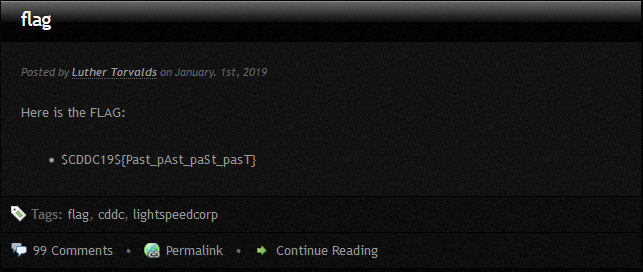
\includegraphics[width=110mm]{figures/osintred/r1.png} \vspace{5mm}
			\caption{The flag is clearly visible}
		\end{figure}

	% end subsection

	\subsection{Flag}
		The flag for this challenge was \cddcflag{Past\_pAst\_paSt\_pasT}.
	% end subsection

% end section


\pagebreak
\section{[R-2] I'm Sho Done With This}

	\subsection{Solution}

		The hint was in the question title itself --- turns out that there is a search engine called \enquote{ShoDan}
		\footnote{\url{https://www.shodan.io}}, which claims to be the world's first search engine for internet connected devices.

		Sure enough, searching for our favourite company \enquote{lightspeedcorp} yielded the following results:

		\begin{figure}[!htbp]\centering
			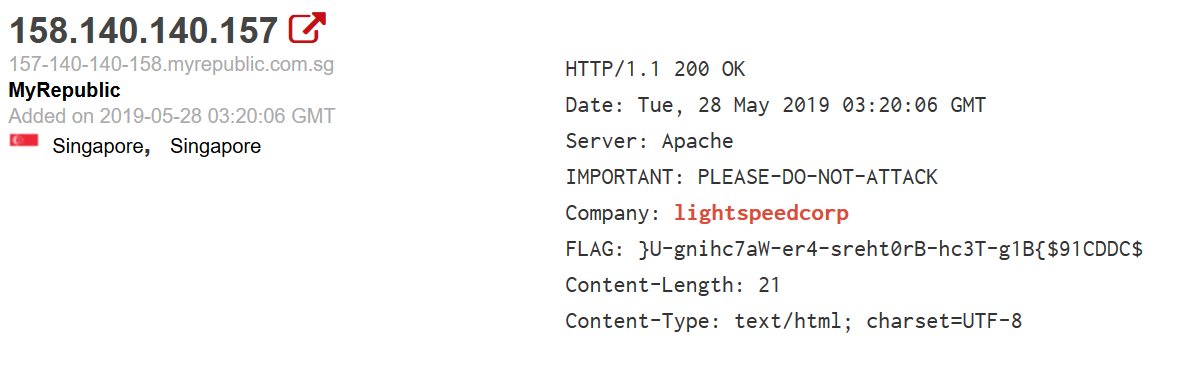
\includegraphics[width=150mm]{figures/osintred/r2.png} \vspace{5mm}
			\caption{The flag is reversed, for some reason}
		\end{figure}

		A trivial string-reverse later, the flag is obtained.

	% end subsection

	\subsection{Flag}
		The flag for this challenge was \cddcflag{B1g-T3ch-Br0thers-4re-Wa7ching-U}.
	% end subsection


% end section

















\pagebreak\part{OSINT\_BLUE}
% b0, b1, b2, b3-1, b3-2, b4-1, b4-2

\section{[B-0] What's in, Doc?}


% end section



\section{[B-1] Fight the Binary Monster}

% end section


\section{[B-2] I <3000 PHISH}

% end section


\section{[B-3-1] Onion Sauce}

% end section


\section{[B-3-2] When Your ZIL Turns to NIL}

% end section


\section{[B-4-1] Where I Get All My GIFs From}

% end section


\section{[B-4-2] Hide N Seek}

% end section


\pagebreak\part{Programming}
% count1, count2, count4.

\section{Count 1: Baby}

	This was a fairly simple code golfing challenge; inspection of the provided \ttt{count1-baby.py} file
	gave the character limit as \num{53} characters. The starting code is given as this:

	\begin{listing}[!htbp]
		\begin{ccode}
			#include <stdio.h>

			int main(int argc, char *argv[])
			{
				int i;

				for( i = 1 ; i < 10000 ; i++ )
				{
					printf("%d,", i);
				}

				return 0;
			}
		\end{ccode}
	\end{listing}

	\subsection{Solution}

		Compiling and running the program shows that the expected output of the minified program are the numbers \ttt{1} to \ttt{9999},
		separated by commas (with a trailing comma after \ttt{9999}).

		Besides the obvious steps like removing whitespace and newlines, knowledge of the C standard and ignorance of compiler warnings
		can yield the following transformations:

		\begin{bulletlist}
			& \ttt{printf} is an implicitly defined standard library function; \ttt{stdio.h} can be removed
			& Functions do not require a type specifier; \ttt{int main} can be shortened to \ttt{main}
			& \ttt{main} does not need to take arguments, leaving \ttt{main()}
			& The verifier rejects spaces, so \ttt{int i} has to be changed to \ttt{int(i)} (which is valid)
			& \ttt{main} does not need to explicitly \ttt{return 0}
		\end{bulletlist}

		\pagebreak
		This yields the final program, at \num{53} characters long:

		\begin{listing}[!htbp]\begin{ccode}
			main(){int(i);for(i=1;i<10000;i++){printf("%d,",i);}}
			\end{ccode}
			\caption{The solution for Count 1: Baby}
			\label{code:count1}
		\end{listing}

	% end subsection

	\subsection{Flag}

		The flag for this challenge was \cddcflag{Count2\_is\_waiting\_Please\_enjoy!}.

	% end subsection

% end section



\pagebreak
\section{Count 2: Wildness}

	The required output for this challenge is the same as the previous challenge (Count 1: Baby), but the restrictions have been
	tightened. This time, OP's friend \enquote{doesn't like to go wild}, or, in other words, the following characters cannot be
	used in the source code: \ttt{<== w1lD ==>}. Additionally, the character limit has been reduced to \num{41}.

	\subsection{Solution}

		Starting from the code for Count 1 (Listing \ref{code:count1}), we can apply some more non-obvious tricks:

		\begin{bulletlist}
			& Variables don't need a type specifier, and will default to \ttt{int}
			& Variables with static storage duration will be initialised to \ttt{0} (obviating the need for \ttt{=})
			& \ttt{!=} is equivalent to a bitwise XOR (\ttt{\^{}}) for integers (removing \ttt{<})
			& Taking advantage of \ttt{i++} semantics can replace \ttt{1e4} with \ttt{9999} (since \ttt{1} can't be used)
		\end{bulletlist}

		This yields the final program, again at exactly \num{41} characters:

		\begin{listing}[!htbp]\begin{ccode}
			i;main(){for(;i++^9999;printf("%d,",i));}
			\end{ccode}
			\caption{The solution for Count 2: Wildness}
		\end{listing}

	% end subsection

	\subsection{Flag}

		The flag for this challenge was \cddcflag{This\_really\_helps\_m3\_a\_lot}

	% end subsection

% end section



\pagebreak
\section{Count 4: Madness - Filter}

	For this challenge, the character limit is slightly relaxed to \num{44} characters, but OP's friend has a faulty keyboard now,
	and all lowercase characters except those in \enquote{\ttt{mad printf}} (\enquote{a}, \enquote{d}, \enquote{f}, \enquote{i}, \enquote{m},
	\enquote{n}, \enquote{p}, \enquote{r}, and \enquote{t}) cannot be used.

	\subsection{Solution}

		Given that all the looping constructs (\ttt{for}, \ttt{while}, and even \ttt{goto}) cannot be used due to having illegal characters,
		the only logical solution is recursion.

		\begin{bulletlist}
			& It is not illegal to call \ttt{main} recursively
			& When called with no arguments, \ttt{argc} is \ttt{1}; so \ttt{main(i)} will initialise \ttt{i} to \ttt{1}
			& \ttt{1E4} is equally as valid as \ttt{1e4}, which is identical to \ttt{10000}
			& The first arm of the ternary operator can be omitted: \ttt{x?:y} is valid.
		\end{bulletlist}

		We came up with two independent solutions to this problem:

		\begin{listing}[!htbp]\begin{ccode}
			main(i){printf("%d,",i++);if(i<1E4)main(i);}
			\end{ccode}
			\caption{The solution for Count 2: Wildness}
		\end{listing}

		\begin{listing}[!htbp]\begin{ccode}
			i;main(){printf("%d,",++i);i>=9999?:main();}
			\end{ccode}
			\caption{An alternative solution for Count 2: Wildness}
		\end{listing}

		In both cases, the code was exactly \num{44} characters long.

	% end subsection

	\subsection{Flag}

		The flag was \cddcflag{Main\_might\_be\_just\_a\_function\_but\_it\_is\_really\_special!}.

	% end subsection

% end section

















\pagebreak\part{Reverse Engineering}

\section{LSCVM: Immaculate Invasion}

	\subsection{Solution}

		\newcommand{\ttoc}[1]{\ttt{\bld{#1}}}

		The tool of choice for this challenge was \itl{Cutter}\footnote{\url{https://github.com/radareorg/cutter}}, an open-source
		reverse-engineering framework which performs disassembly, function analysis, and function/value renaming, among other things.

		\begin{figure}[!htbp]\centering
			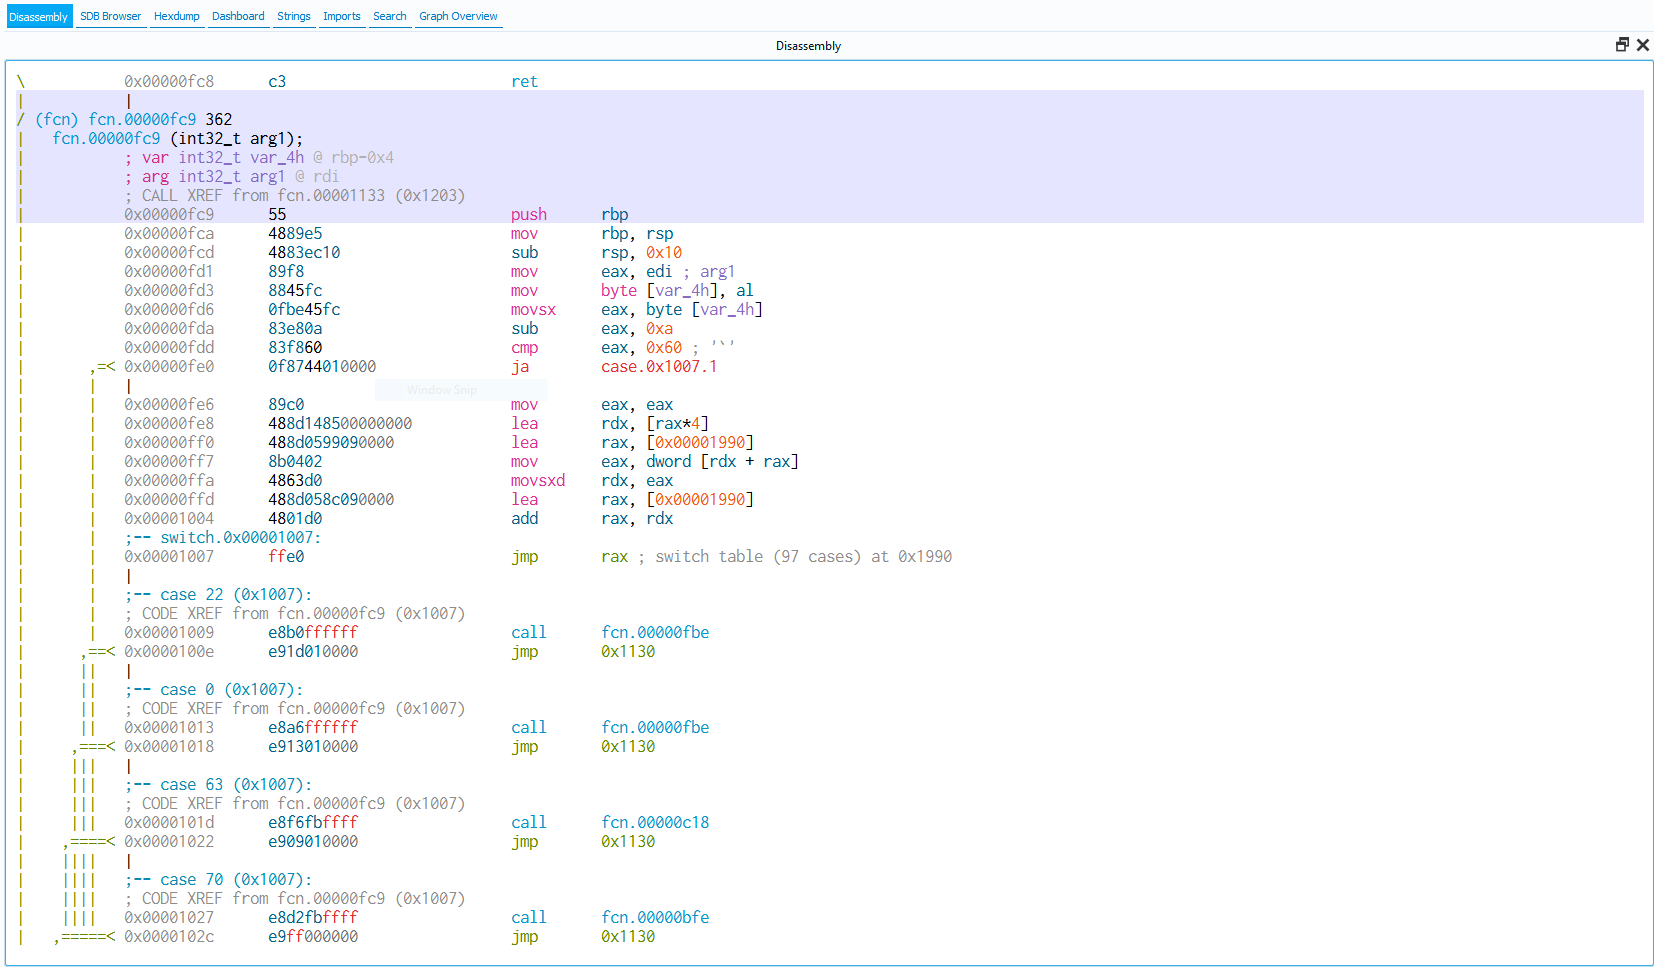
\includegraphics[width=150mm]{figures/lscvm-ii/cutter-screenshot.png} \vspace{5mm}
			\caption{A screenshot of Cutter}
			\label{fig:jumptable}
		\end{figure}

		The first hurdle was getting the program to run beyond its error message of \ttt{[-] Flag file open error}; upon
		inspection of the disassembly, the program tries to open a file named \enquote{flag}, which presumably contains the
		flag on the server-side --- \mintinline{sh}{$ touch flag} convinced the program to start.

		\pagebreak
		Given that the program asks for a login ID, the next step was to check for strings and \ttt{strcmp}s in the code,
		and one was indeed found:

		\begin{figure}[!htbp]\centering
			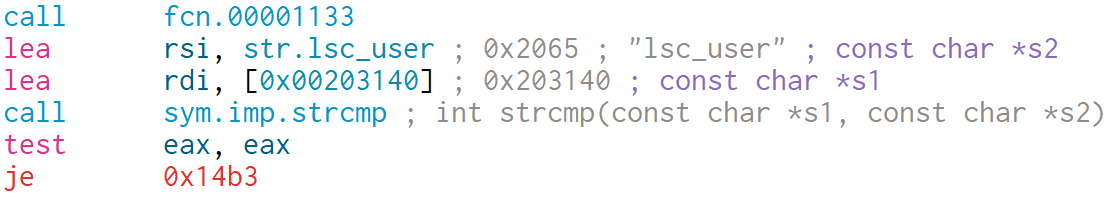
\includegraphics[width=150mm]{figures/lscvm-ii/user-strcmp.png} \vspace{5mm}
			\caption{A suspicious \ttt{strcmp}}
		\end{figure}

		Of course, no challenge is so easy, especially one that sat at above 950 points more than 24 hours after the qualifiers started. On
		further inspection, the operand of \ttt{strcmp} appeared to be the output of a call to \ttt{fcn.00001133}, which itself
		took some very long and suspicious strings as input: \ttt{eiMaAghMcAgjcMMdAgjcMMaAgjcMMaAhhcMMdAijMaAcfMPPPPPPPP}.

		Another discovery was this instruction: \ttt{nasm}{cmp dword [var\_1174h], 2}, where \ttt{var\_1174h} contained the value
		of \ttt{argc}. Passing a second argument in the invocation (eg. \mintinline{sh}{$ ./lscvm-ii x}) revealed a \itl{very} useful
		debugging mode that printed what appeared to be a stack.

		Following the call chain eventually led to the jump table for opcode dispatch, pictured in Figure \ref{fig:jumptable}. Some quick
		analysis revealed that this was a indeed stack-based virtual machine (\itl{thankfully}). Combined with the debugging output, and the
		fact that the text output (the banner, login prompt, etc.) was printed using the VM instead of say \ttt{printf}, some basic opcodes
		were decoded:

		\begin{nicetable}[1.3][0.6\textwidth]{ X[c,m] | X[c,m] | X[c,m] | X[3,c,m] }
			Opcode              &   Pops            &   Pushes              &   Description \\ \hline
			\ttoc{u} to \ttoc{u}&   --              &   \ttt{0} to \ttt{9}  &   constant    \\
			\ttoc{A}            &   \ttt{a}, \ttt{b}&   \ttt{a + b}         &   add         \\
			\ttoc{M}            &   \ttt{a}, \ttt{b}&   \ttt{a * b}         &   multiply    \\
			\ttoc{P}            &   \ttt{a}         &   --                  &   \ttt{printf("\%c",a)} \\
		\end{nicetable}

		Piecing things together, it was inferred that we were most likely supposed to input a \itl{program} when asked for the user ID,
		which would then print \ttt{lsc\_user} as required. Given that ASCII values for the lowercase alphabets start at 97, a small
		program was quickly written that would take in a string and output opcodes that would print it (Listing \ref{code:lscvm-deasciiinator}).

		After trying it out, however, we were quickly met with disappointment, as we were faced with our old friend \ttt{[-] Wrong id}.

		\pagebreak
		After more digging, the user id was expected to be at the memory address \ttt{0x203140}; using the renaming feature of Cutter, we could
		make it easier to spot:

		\begin{figure}[!htbp]\centering
			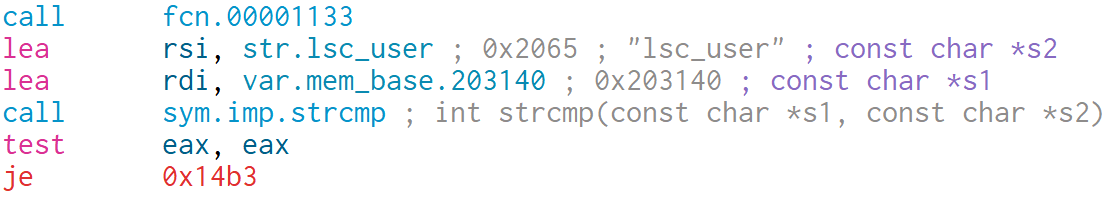
\includegraphics[width=150mm]{figures/lscvm-ii/addr-after-rename.png} \vspace{5mm}
			\caption{\ttt{[0x203140]} after being renamed into \ttt{var.mem\_base.203140}}
		\end{figure}

		Scrolling through the opcode list while looking for the address (now renamed) yielded this very interesting function, mapped to opcode
		\ttt{K}:

		\begin{figure}[!htbp]\centering
			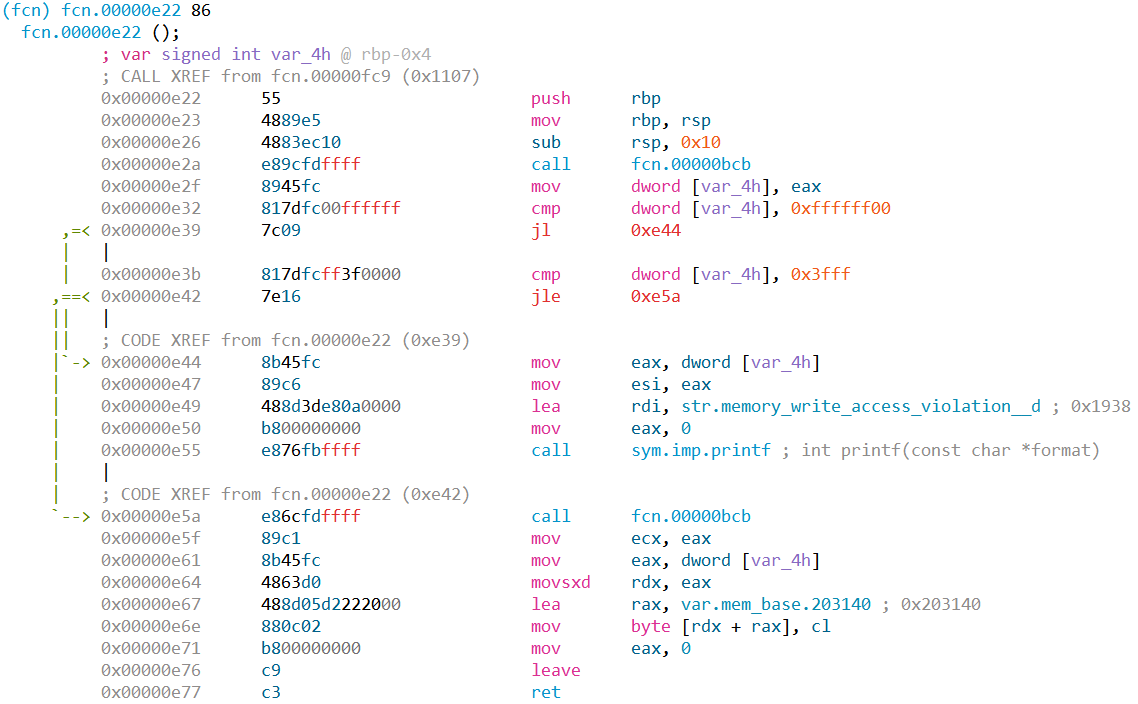
\includegraphics[width=150mm]{figures/lscvm-ii/write-to-memory.png} \vspace{5mm}
			\caption{A function to \sout{surpass metal gear} write to memory?}
		\end{figure}

		There was also an accompanying opcode \ttoc{E}, which read a value from memory. The memory buffer appeared to be an array of 32-bit
		values, and opcodes \ttoc{K} and \ttoc{E} took an index into this array. Slight modifications were made to \ttt{lscvm-deasciiinator}
		to yield \ttt{lscvm-memoryinator} (basically keeping track of an offset and replacing \enquote{P} with \enquote{K}), which would
		generate opcodes to write a string into a given offset in memory.

		\pagebreak
		Finally, then, the challenge could be solved (the password was also in plain sight, \ttt{hi\_darkspeed-corp!}):

		\begin{listing}[!htbp]
			\begin{minted}[autogobble,xleftmargin=0.075\textwidth,xrightmargin=0.075\textwidth,frame=leftline,framesep=4mm,framerule=0.4mm]{sh}
				$ ./lscvm-memoryinator
				string: lsc_user
				address: 0

				ggdMMaKfgAfMcMfAbKjjMjAjAcKgfdMMfAdKfgAfMcMhAeKfgAfMcMfAfKcf
				McfMMbAgKfgAfMcMeAhK

				string: hi_darkspeed-corp!
				address: 0

				jeAiMaKhdfMMbKgfdMMfAcKcfMcfMMdKjjMjAhAeKfgAfMcMeAfKhdfMMcAg
				KfgAfMcMfAhKfgAfMcMcAiKcfMcfMMbAjKcfMcfMMbAcfMKcfMcfMMbcfMMb
				AKfddMMbcfMMcAKjjMjAjAbcfMMdAKfgAfMcMbAbcfMMeAKfgAfMcMeAbcfM
				MfAKfgAfMcMcAbcfMMgAKfgAdMbcfMMhAK
				^C

				$ nc lscvm-ii.cddc19q.ctf.sg 9001

				=== Welcome to LSCVM(LightSpeed Corp Virtual Machine) ===
				ID : ggd...AhK
				Password : jeA...hAK

				Login Successful! $CDDC19${IcY_GrE37ings_Fr0M_LigHT5pEeDC0Rp}

				lsc_user, Good Bye!
			\end{minted}
		\end{listing}

	% end subsection


	\subsection{Flag}
		The flag for this challenge was \cddcflag{IcY\_GrE37ings\_Fr0M\_LigHT5pEeDC0Rp}.
	% end subsection


	\subsection{Further Analysis}
		While we were unable to actually come up with a quine to submit for the next LSCVM challenge (Quintessential Harlequin), we
		continued to take apart the VM (on the advice that it would be used again in the Finals!), since solving \ttt{lscvm-ii} did
		not require all of the opcodes (far from it).

		Again, the renaming feature of Cutter was extremely helpful, and we were able to discover the address of the program counter, the
		base address of the stack, and (in the case of \ttt{lscvm-qh}), the mirror of stdout. Each buffer appears to be a identical
		with a fixed size of \ttt{0x4e200} bytes (\ttt{0x13880} 32-bit words), and the number of items stored after the last
		element (ie. at offset \ttt{0x4e200} from the base address).

		We (eventually) managed to decipher all of the opcodes and their purpose:


		\begin{nicetable}[1.3][0.9\textwidth]{ X[.7,c,m] | X[c,m] | X[c,m] | @{\hspace{1.5em}}X[3,l,m] }
			Opcode              &   Pops                &   Pushes              &   \multicolumn{1}{c}{Description} \\ \hline
			\ttoc{a} to \ttoc{j}&   --                  &   \ttt{0} to \ttt{9}  &   constant                                    \\
			\ttoc{A}            &   \ttt{a}, \ttt{b}    &   \ttt{a + b}         &   add                                         \\
			\ttoc{B}            &   --                  &                       &   stop execution immediately                  \\
			\ttoc{C}            &   \ttt{x}             &   --                  &   call (jump to absolute instruction \ttt{x}) \\
			\ttoc{D}            &   \ttt{x}             &   --                  &   pop (drop)                                  \\
			\ttoc{E}            &   \ttt{addr}          &   \ttt{value}         &   read memory from \ttt{addr}                 \\
			\ttoc{F}            &   \ttt{ofs}           &   \ttt{value}         &   fetch from stack (\ttt{ofs} elms below top) \\
			\ttoc{G}            &   \ttt{ofs}           &   --                  &   relative jump forward                       \\
			\ttoc{H}            &   \ttt{ofs}           &   \ttt{value}         &   same as \ttoc{F}, but removes the element   \\
			\ttoc{I}            &   \ttt{x}             &   --                  &   \ttt{printf("\%d",x)}                       \\
			\ttoc{J}            &   \ttt{a}, \ttt{b}    &   \ttt{cmp}           &   $-1$ if $a<b$, $0$ if $a=b$, $1$ if $a>b$   \\
			\ttoc{K}            &   \ttt{val}, \ttt{addr}&  --                  &   writes \ttt{val} to memory at \ttt{addr}    \\
			\ttoc{M}            &   \ttt{a}, \ttt{b}    &   \ttt{a * b}         &   multiply                                    \\
			\ttoc{P}            &   \ttt{x}             &   --                  &   \ttt{printf("\%c",x)}                       \\
			\ttoc{R}            &   --                  &   --                  &   return                                      \\
			\ttoc{S}            &   \ttt{a}, \ttt{b}    &   \ttt{a - b}         &   subtract                                    \\
			\ttoc{V}            &   \ttt{a}, \ttt{b}    &   \ttt{a / b}         &   integer divide                              \\
			\ttoc{Z}            &   \ttt{cond}, \ttt{ofs}&  --                  &   jump (relative) if \ttt{cond} is $0$
		\end{nicetable}

		Of note are the \ttoc{C} and \ttoc{R} opcodes, which \itl{call} and \itl{return} respectively. There is another array which
		is only accessed by these instructions that functions as a \itl{callstack}. \ttoc{C} pushes the current program counter ($PC$)
		to this callstack, and \ttoc{R} pops the return address from the callstack, and sets $PC$ to it, moving execution back to the
		callsite.


		% \undef\ttoc


	% end subsection


% end section




















\pagebreak\part{Miscellaneous}
% polyglot, very serious, fancy numbers

% ufgh
\newfontscript{Devanagari}{deva,dev2}
\newfontface{\hindi}[Script=Devanagari]{Lohit-Devanagari}

\section{Polyglot}

	\subsection{Solution}

		The obvious solution was to put each sentence into Google Translate\footnote{\url{https://translate.google.com}};
		all 10 sentences were some variation of \enquote{the first letter of this language is the flag}. Coupled with
		the input format, given as \ttt{[01][02]\~[03][04][05][06]\&[07][08][09][10]!}, we were able to decode the
		flag.

		\begin{nicetable}[1.3][0.95\textwidth]{ X[.5,c,m] | X[.7,c,m] | X[3.5,c,m] }
			Number  &   Language    &   Sentence                      \\ \hline
			\ttt{01}&   Hindi       &   {\hindi इस भाषा का पहला चरित्र झंडा बनाता है। }\\
			\ttt{02}&   Indonesian  &   Karakter pertama bahasa ini yang mengibarkan bendera.\\
			\ttt{03}&   Chinese     &   这种语言的第一个字符构成了旗帜。\\
			\ttt{04}&   Dutch       &   Het eerste teken van deze taal vormt de vlag. \\
			\ttt{05}&   Danish      &   Det første tegn på dette sprog udgør flag. \\
			\ttt{06}&   Catalan     &   El primer caràcter d'aquest idioma constitueix la bandera. \\
			\ttt{07}&   Norwegian   &   Det første tegnet av dette språket utgjør flagget. \\
			\ttt{08}&   Spanish     &   El primer carácter de este lenguaje lo constituye la bandera. \\
			\ttt{09}&   Hmong       &   Thawj qhov cim ntawm hom lus no ua rau tus chij. \\
			\ttt{10}&   Croatian    &   Prvi znak ovog jezika čini zastavu.
		\end{nicetable}

		Assembled, the message was \ttt{HI\~{}CDDC\&NSHC}; it helped that there was a coherent message to verify that
		Google Translate didn't misdetect any of the langauges.

	% end subsection

	\subsection{Flag}
		The flag for this challenge was \cddcflag{HI\~{}CDDC\&NSHC}.
	% end subsection

% end section


% lmao welcome to overkill land
% all because yudong wants to draw a block diagram
\ExplSyntaxOn
\NewDocumentCommand{\dopininparse}{m m}{
	\node [right, font=\scriptsize] at (\str_use:N\chipname.bpin~ \int_eval:n{#1 + 1}) {\hspace{0.5mm}\texttt{#2}};
	\draw (\str_use:N\chipname.pin~ \int_eval:n{#1 + 1}) node[inputarrow,right]{};
	\coordinate(\str_use:N\chipname-i#1) at (\str_use:N\chipname.pin~ \int_eval:n{#1 + 1});
}
\NewDocumentCommand{\dopinoutparse}{m m}{
	\node [left=-0.5mm, font=\scriptsize] at (\str_use:N\chipname.bpin~ \int_eval:n{\numpins - #1}) {\texttt{#2}};
	\draw (\str_use:N\chipname.pin~ \int_eval:n{\numpins - #1}) node[inputarrow,right]{};
	\coordinate (\str_use:N\chipname-o#1) at (\str_use:N\chipname.pin~ \int_eval:n{\numpins - #1});
}

% position, pins count, node name, label, input pins, output pins, optional args.
\NewDocumentCommand{\drawchip}{ m m m m m m O{} }{%
	\draw #1 node[dipchip, hide~ numbers, no~ topmark, anchor=pin~ 1, num~ pins=#3, #7](#2){};
	\node [above, font=\small] at (#2.north) {\texttt{#4}};

	\str_clear_new:N \chipname
	\str_set:Nn \chipname {#2}

	\int_zero_new:N \numpins
	\int_set:Nn \numpins {#3}

	\keyval_parse:NNn{\use_none:n}{\dopininparse}{#5}
	\keyval_parse:NNn{\use_none:n}{\dopinoutparse}{#6}
}

\def\splicept{coordinate(splpt){}node[splicept]{}}
\ExplSyntaxOff

\tikzset{
	splicewire/.style 2 args={
		midway,fill=white,inner sep=-0.5mm,outer sep=0mm,
		node contents={\scriptsize\texttt{[#1:#2]}}
	},
	splicept/.style={ coordinate, diamondpole, circuitikz/bipoles/length=20mm },
	splitpt/.style ={ circ },
	openwire/.style={ line width=0.2mm, ocirc, circuitikz/bipoles/length=25mm },
	circuitikz/nodes width=0.025,
	circuitikz/multipoles/thickness=1.5,
	circuitikz/multipoles/dipchip/width=1.4,
	circuitikz/multipoles/external pins width=0,
	circuitikz/multipoles/dipchip/pin spacing=0.25,
	circuitikz/multipoles/external pins thickness=0
}


\section{Super Strong TeleVision}

	With the obvious hints in the challenge statement, we got to work decoding.

	SSTV, or Slow Scan Television, is a picture transmission method used mainly by amateur radio operators to transmit and receive static pictures
	via radio in monochrome or colour\footnote{\url{en.wikipedia.org/wiki/Slow-scan_television}}. It can also be used to hide easter\footnote{
	\url{https://wiki.kerbalspaceprogram.com/wiki/List_of_easter_eggs}} eggs\footnote{\url{https://half-life.fandom.com/wiki/Portal_ARG}}...

	\subsection{Solution}

		% https://www.chonky.net/hamradio/decoding-sstv-from-a-file-on-a-linux-system
		The solution was rather straightforward. Using \itl{PulseAudio} as a link between \itl{VLC} and
		\itl{QSSTV}\footnote{\url{http://users.telenet.be/on4qz/qsstv/index.html}} (an open-source Linux SSTV application), we were able to rather quickly decode
		the SSTV image:

		\begin{figure}[!htbp]
			\centering
			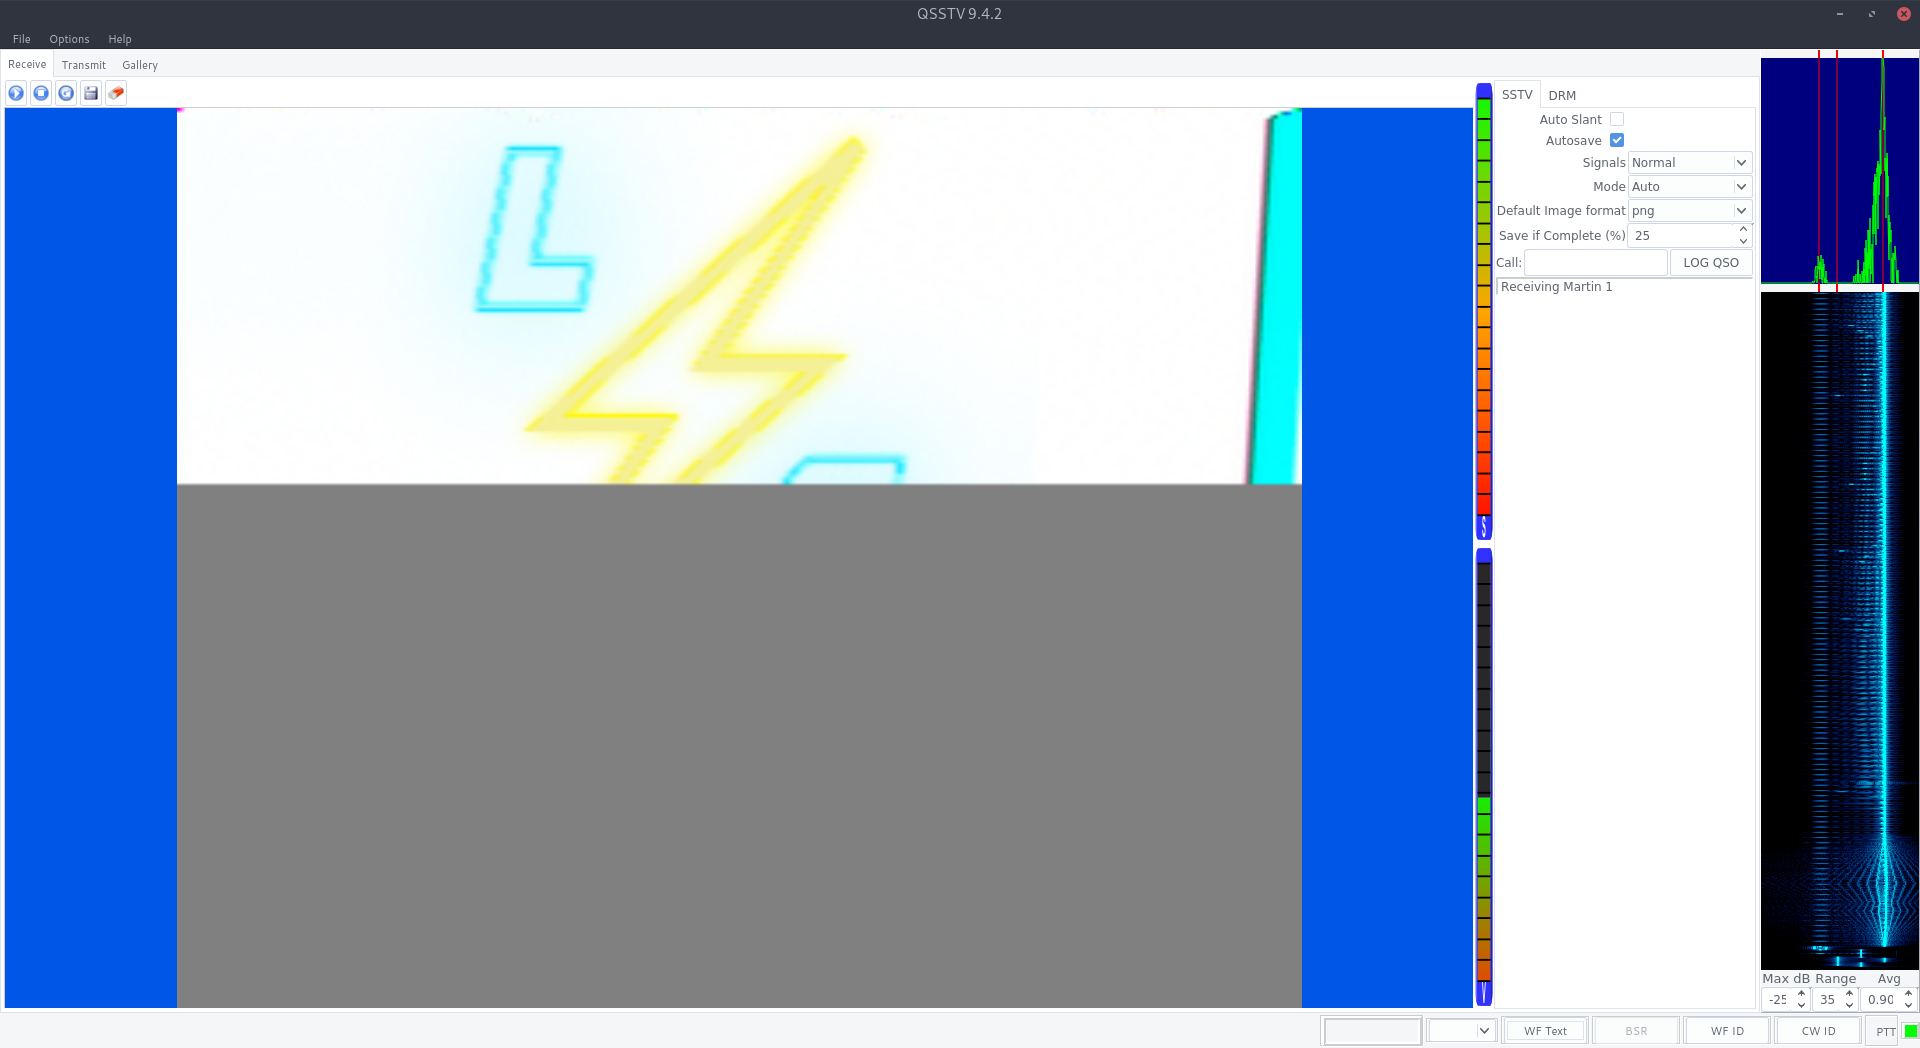
\includegraphics[width=150mm]{figures/sstv/QSSTV.png} \vspace{5mm}
			\caption{QSSTV decoding the image; its frequency spectrum can be seen on the right}
		\end{figure}

		\pagebreak
		In this case, \itl{PulseAudio} acted as the pipe that redirects the \ttt{.wav} file as an input into the \itl{QSSTV} decoder:

		\begin{figure}[!htbp]\centering
			\begin{circuitikz}
				\drawchip{(1, 0)}{vlc}{6}{VLC}{
					1=\empty}{1=\empty
				}[circuitikz/multipoles/dipchip/width=1]

				\drawchip{(4, 0)}{pulseaudio}{6}{PulseAudio}{
					1=\empty}{1=\empty
				}[circuitikz/multipoles/dipchip/width=1]

				\drawchip{(7, 0)}{qsstv}{6}{QSSTV}{
					1=\empty}{1=\empty
				}[circuitikz/multipoles/dipchip/width=1]

				% draw backwards...
				\draw[line width=.4mm] (vlc-i1) -- ++(-1, 0) node[anchor=mid east]{.wav file} {};
				\draw[line width=.4mm] (vlc-o1) -- (pulseaudio-i1) {};
				\draw[line width=.4mm] (pulseaudio-o1) -- (qsstv-i1) {};
				\draw[line width=.4mm] (qsstv-o1) -- ++(1.2, 0) node[anchor=west,inputarrow]{} ++(.1,0) node[anchor=mid west]{image} {};


			\end{circuitikz}\vspace{5mm}
			\caption{Data Pipeline Setup}
		\end{figure}
	
		This works by enabling and making use of the default \ttt{null-sink} provided with every \itl{PulseAudio} installation:
		
		\begin{minted}[autogobble,xleftmargin=0.075\textwidth,xrightmargin=0.075\textwidth,frame=leftline,framesep=4mm,framerule=0.4mm]{sh}
			pactl load-module module-null-sink sink_name=virtual-cable
			pavucontrol
		\end{minted}
	
		and making \itl{QSSTV} record from the \ttt{null sink}:
		
		\begin{figure}[!htbp]
			\centering
			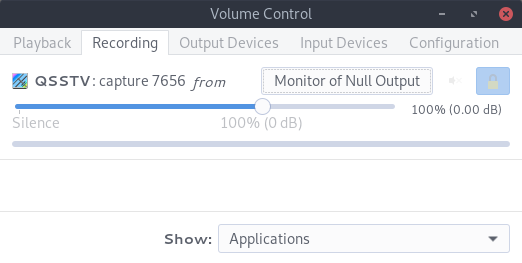
\includegraphics[width=150mm]{figures/sstv/pavu.png} \vspace{5mm}
			\caption{QSSTV -- Record from the \ttt{null-sink}}
		\end{figure}
		
		Once everything is set up, we simply start recording on \itl{QSSTV} and use \itl{VLC} to playback the \ttt{.wav} file to the \ttt{null-sink} and watch the magic unfold.
	% end subsection

	\subsection{Flag}
		After some suspense as the SSTV audio played back in real time, the image was fully decoded, revealing the flag, which
		was \cddcflag{Light\$peedCorp-\$\$TV}.

		\begin{figure}[!htbp]\centering
			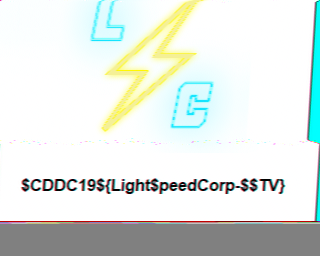
\includegraphics[width=80mm]{figures/sstv/SSTV.png} \vspace{5mm}
			\caption{Decoded SSTV Image}
		\end{figure}
	% end subsection
% end section



\makeatletter\@addtoreset{section}{part}\makeatother
\pagebreak\part{Appendix}
\section{Code Listings}

	\subsection{\texttt{lscvm-memoryinator}}
		\vspace{\baselineskip}
		\begin{multipagecode}
			\inputminted[xleftmargin=0.075\textwidth,xrightmargin=0.075\textwidth,frame=leftline,framesep=4mm,framerule=0.4mm,
	linenos=true]{cpp}{../lscvm/lscvm-memoryinator.cpp}
			\caption{lscvm-memoryinator.cpp}
			\label{code:lscvm-memoryinator}
		\end{multipagecode}
	% end subsection
% end section

\end{document}

























